% !TEX encoding = UTF-8
% !TEX TS-program = pdflatex
% !TEX root = ../tesi.tex

\renewcommand\theadalign{cb}
\renewcommand\theadfont{\bfseries}
\renewcommand\theadgape{\Gape[4pt]}
\renewcommand{\arraystretch}{2}

%**************************************************************
\chapter{Descrizione dello stage}
\label{cap:descrizione-stage}
%**************************************************************

\intro{Questo capitolo descrive in dettaglio lo stage. Ne specifica il progetto da svolgere contestualizzandolo nella realtà aziendale, i requisiti richiesti, gli obiettivi da raggiungere e la pianificazione iniziale.}\\

%**************************************************************
\section{Introduzione al progetto e contestualizzazione}
Nel contesto del supply chain management in cui l’azienda opera, ha assunto una gran rilevanza l’organizzazione dei turni di singoli lavoratori o di squadre di lavoratori, in relazione alle competenze da loro possedute e richieste dai vari lavori da portare a compimento. \\ \\
Il progetto di stage si prefiggeva l'obiettivo di estendere per la risoluzione dei problemi di scheduling il \emph{\gls{framework}}\glsfirstoccur\ aziendale e scrivere un'applicazione che lo utilizzasse andando a risolvere un problema specifico. L'obiettivo finale è utilizzare il framework per lo scheduling delle squadre dei meccanici, tuttavia è stato deciso che, per cominciare a studiare i problemi di scheduling e la fattibilità di risolverli con metodi \emph{\gls{algeur}}\glsfirstoccur\ e \emph{\gls{meteur}}\glsfirstoccur, fosse opportuno cominciare da un problema più semplice: l'organizzazione dei turni nei casinò. L'organizzazione dei turni dei meccanici sarà il naturale proseguimento di questo progetto, e la complessità maggiore dovuta allo schedulazione di individui singoli inseriti in un gruppo anch'esso da schedulare sarà supportata dal framework di base, robusto e già testato, sviluppato all'interno del progetto di stage. \\ 
Il problema della schedulazione dei turni all'interno dei casinò è stato scelto come problema di partenza in quanto comunque di interesse per l'azienda, che ha contatti con un manager de ``The Hippodrome Casino'' di Londra, il quale ha sottoposto il problema in quanto, al momento, lo scheduling viene fatto completamente a mano, dovendo tenere conto di numerosi vincoli e variabili. \\

%**************************************************************
\section{Vincoli}
È stato concordato con \TS\ che lo stage fosse svolto presso la sede operativa della stessa, ad Albignasego, affinché io potessi essere inserita nel contesto aziendale ed avere la possibilità di confrontarmi col resto del team di sviluppo in maniera immediata. \\
Il tutor aziendale ha richiesto di scrivere ogni giorno un breve report delle attività svolte, delle difficoltà incontrate, degli obiettivi raggiunti e delle considerazioni personali su un documento condiviso su \emph{\gls{drive}}\glsfirstoccur, ha inoltre richiesto che ogni mattina prima di cominciare a lavorare si svolgesse una breve riunione con tutto il team per focalizzarsi sulle attività della giornata.\\
Lo stage, che prevede una durata di 300 ore, è stato pianificato su una durata di poco meno di 9 settimane prevedendo in media 6.5 ore lavorative al giorno. Tale stima è stata effettuata al ribasso per permettere una certa flessibilità per quanto riguarda l'orario di lavoro e/o eventuali giorni liberi che avrei potuto prendere per impegni universitari; l'orario di lavoro invece è stato stabilito dal lunedì al venerdì, dalle 9.00 alle 18.00 con un'ora di pausa pranzo. \\
Prima dell'inizio dello stage \TS\ ha redatto un piano di lavoro in cui sono stati fissati gli obiettivi e la pianificazione settimanale per lo stage, che vengono illustrati nei paragrafi ``Obiettivi'' e ``Pianificazione'' di questo capitolo. \\
Per quanto riguarda i vincoli tecnologici, essi saranno trattati nel paragrafo ``Ambiente di lavoro'' di questo capitolo.
%**************************************************************
\section{Obiettivi}
Sono riportati di seguito gli obiettivi fissati per lo stage con rispettivo identificativo, importanza e breve descrizione. \\
\\
L'identificativo (in breve, Id) è la sigla che identifica ogni requisito e rispetta la notazione \textit{[Importanza][Identificativo]}, dove l'importanza è la sigla \textbf{Ob} / \textbf{De} / \textbf{Op} a seconda che l'obiettivo sia obbligatorio, desiderabile o opzionale; l'identificativo è un numero progressivo che identifica in modo univoco l'obiettivo. \\
\\
Un obiettivo è classificato, secondo l'importanza, come:
    \begin{itemize}
        \item \textbf{Obbligatorio:} è l'importanza attribuita agli obiettivi il cui soddisfacimento dovrà necessariamente avvenire in quanto sono di importanza fondamentale per la riuscita del progetto;
        \item \textbf{Desiderabile:} è l'importanza attribuita agli obiettivi il cui soddisfacimento non è necessario, tuttavia desiderabile;
        \item \textbf{Opzionale:} è l'importanza attribuita agli obiettivi il cui soddisfacimento è del tutto opzionale in quanto renderebbero il progetto più completo.
    \end{itemize}%

\noindent
Nel {\hyperref[cap:conclusioni]{settimo capitolo}}
è riportato un consuntivo che riporta quanti degli obiettivi riportati di seguito sono stati soddisfatti nel corso dello stage.

\begin{center}
\begin{table}[!htb]
    \caption{Obiettivi da raggiungere a fine stage}
    \label{tab:obiettivi}
    \begin{tabularx}{\textwidth}{|c|c|X|}
        \hline
        \thead{ID} & \thead{IMPORTANZA} & \thead{DESCRIZIONE}\\
        \hline \hline
        Ob1 & Obbligatorio & Assimilazione dei concetti di base dei problemi di scheduling \\
        \hline
        Ob2 & Obbligatorio & Definizione del problema di scheduling da risolvere \\
        \hline
        Ob3 & Obbligatorio & Studio della letteratura scientifica sui modelli e i metodi per problemi di schedulazione e indagine sugli algoritmi euristici più adatti al tipo di problema in esame \\
        \hline
        Ob4 & Obbligatorio & Studio del framework aziendale dalla relativa documentazione \\
        \hline
        Ob5 & Obbligatorio & Progettazione di un algoritmo euristico per la soluzione del problema \\
        \hline
        Ob6 & Obbligatorio & Implementazione prototipale dell’algoritmo euristico \\
        \hline
        Ob7 & Obbligatorio & Integrazione dell’algoritmo euristico nelle librerie dell’azienda \\
        \hline
        Ob8 & Obbligatorio & Test preliminare su istanze benchmark di problemi di scheduling \\
        \hline
%    \end{tabularx}
%\end{table}%

%\begin{table}[!htb]
%    \begin{tabularx}{\textwidth}{|c|c|X|}
%        \hline
%         \thead{ID} & \thead{IMPORTANZA} & \thead{DESCRIZIONE}\\
%        \hline \hline
        Ob9 & Obbligatorio & Produzione di documentazione sui moduli sviluppati \\
        \hline
        Ob10 & Obbligatorio & Produzione di un manuale di utilizzo dei moduli sviluppati \\
        \hline \hline
        De1 & Desiderabile & Analisi prestazionale su diverse istanze del problema \\
        \hline
        De2 & Desiderabile & Esplorazione di altri contesti applicativi \\
        \hline \hline
        Op1 & Opzionale & Definizione di un modello di programmazione matematica del problema \\
        \hline
        Op2 & Opzionale & Implementazione con AMPL (o altro linguaggio di modellazione matematica) del modello di programmazione lineare intera per la soluzione esatta del problema di scheduling \\
        \hline
    \end{tabularx}
\end{table}%
\end{center}
%**************************************************************
\clearpage
\section{Pianificazione}
La pianificazione del lavoro da svolgere durante lo stage è stata costruita sulla base delle ore di lavoro previste dallo stage curricolare. \\
Il progetto è stato suddiviso in otto periodi:
\begin{enumerate}
    \item \textbf{Analisi del problema.} Periodo di assimilazione dei concetti di base dei problemi di scheduling, per comprenderne contesto e applicazione; approccio al problema dello scheduling nei casinò, con definizione dei vincoli a cui si deve sottostare.
    \item \textbf{Analisi dello stato dell'arte.} Periodo di approfondimento dello studio dei problemi di scheduling, sia nella teoria che nella pratica, con relativi metodi di risoluzione.
    \item \textbf{Ideazione e progettazione di un algoritmo euristico.} Periodo di ricerca di algoritmi euristici per la risoluzione dei problemi di scheduling e di definizione, sulla base di questi ultimi, dello scheletro di un algoritmo per lo scheduling nei casinò.
    \item \textbf{Implementazione dell'algoritmo euristico.} Periodo di familiarizzazione con il framework aziendale, di progettazione dell'architettura da integrare con lo stesso per estenderlo con la risoluzione dei problemi di scheduling, e conseguente implementazione.
    \item \textbf{Integrazione e test dell'algoritmo.} Periodo di implementazione dell'applicazione per il problema specifico dello scheduling nei casinò utilizzando il framework aziendale già esteso; si sono inoltre svolti i primi test semplificati.
    \item \textbf{Confronto con tecniche esatte.} Periodo di studio di modelli matematici per problemi di scheduling classici e definizione di un modello matematico per lo scheduling nei casinò, con conseguente implementazione in \emph{\gls{amplg}}\glsfirstoccur\ e confronto fra \emph{\gls{metodo-esatto}}\glsfirstoccur\ e euristica prodotta.
    \item \textbf{Verifica e testing.} Periodo trasversale ai periodi di Implementazione dell'algoritmo euristico, Integrazione e test dell'algoritmo, Confronto con tecniche esatte. Prevede il testing del prodotto.
    \item \textbf{Produzione di documenti, manuali e relazioni.} Periodo trasversale ai periodi di Ideazione e progettazione di un algoritmo euristico, Implementazione dell'algoritmo euristico, Integrazione e test dell'algoritmo, Confronto con tecniche esatte, Verifica e testing. Prevede la scrittura di documentazione per il codice, comprendente il manuale sviluppatore e il manuale utente; la scrittura di relazioni sui test effettuati e sullo studio del problema.
\end{enumerate}
Di seguito vengono riportate in dettaglio le attività previste per ogni periodo, specificando il numero di ore previste per ognuna e il periodo in cui ne è pianificato lo svolgimento.

%\begin{center}
\begin{table}[!htb]
    \caption{Pianificazione del periodo di stage}
    \label{tab:pdp}
    \begin{tabularx}{\textwidth}{|X|c|c|c|}
        \hline
        \thead{ATTIVITÀ} & \thead{ORE} & \thead{DAL} & \thead{AL}\\
        
        \hline \hline
        \multicolumn{4}{|l|}{\textbf{1. Analisi del problema}}\\
        \hline
        Assimilazione dei concetti di base per problemi di scheduling & 10 & 10/07 & 11/07\\
        \hline
        Definizione delle caratteristiche del problema di scheduling da risolvere & 10 & 11/07 & 12/07\\
        
        \hline \hline
        \multicolumn{4}{|l|}{\textbf{2. Analisi dello stato dell'arte}}\\
        \hline
        Studio della letteratura di base su problemi di scheduling & 15 & 13/07 & 14/07\\
        \hline
        Ricerca ed analisi degli algoritmi più adatti & 15 & 17/07 & 18/07\\
        
        \hline \hline
        \multicolumn{4}{|l|}{\textbf{3. Ideazione e progettazione di un algoritmo euristico}}\\
        \hline
        Individuazione dei blocchi di base da algoritmi pre-esistenti & 15 & 19/07 & 20/07\\
        \hline
        Integrazione dei blocchi & 10 & 21/07 & 24/07\\
        \hline
        Definizione dell’algoritmo di soluzione & 15 & 24/07 & 25/07\\
        
        \hline \hline
        \multicolumn{4}{|l|}{\textbf{4. Implementazione dell'algoritmo euristico}}\\
        \hline
        Studio ed assimilazione del framework aziendale & 15 & 26/07 & 27/07\\
        \hline
        Progettazione dei moduli & 15 & 28/07 & 31/07\\
        \hline
        Implementazione & 40 & 01/08 & 07/08\\
        
        \hline \hline
        \multicolumn{4}{|l|}{\textbf{5. Integrazione e test dell’algoritmo}}\\
        \hline
        Integrazione dell’algoritmo nelle librerie dell’azienda & 30 & 08/08 & 11/08\\
        \hline
        Test preliminari su istanze semplificate & 15 & 21/08 & 22/08\\
       
        \hline \hline
        \multicolumn{4}{|l|}{\textbf{6. Confronto con tecniche esatte}}\\
        \hline
        Studio dei modelli in letteratura & 10 & 23/08 & 24/08\\
        \hline
        Definizione di un modello matematico & 10 & 24/08 & 25/08\\
        \hline
        Implementazione del modello in AMPL & 10 & 28/08 & 29/08\\
        \hline
        Confronto con i risultati dell'euristica e analisi delle presentazioni & 10 & 29/08 & 30/08\\
        
        \hline \hline
        \textbf{7. Verifica e testing} & 20 & 01/08 & 04/09\\
        
        \hline \hline
        \textbf{8. Produzione di documenti, manuali e relazioni} & 35 & 17/07 & 15/09\\
        \hline
        
    \end{tabularx}
\end{table}%
%\end{center}
\clearpage
%[height=25cm ,keepaspectratio]
\begin{figure}[!h]
    \begin{widepage}
    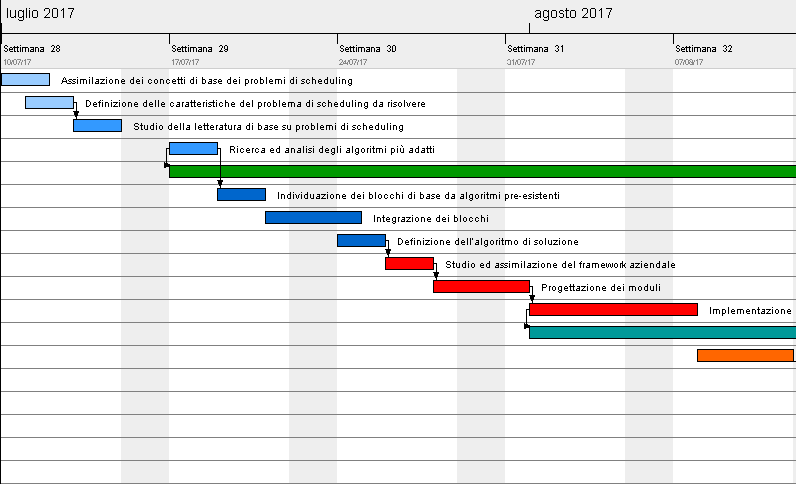
\includegraphics[width=14.9cm,keepaspectratio]{../immagini/pdp_1.png}
    \caption{Diagramma di Gantt per il piano di lavoro, settimane 1-5}
    \end{widepage}
\end{figure}
\begin{figure}[!h]
    \begin{widepage}
    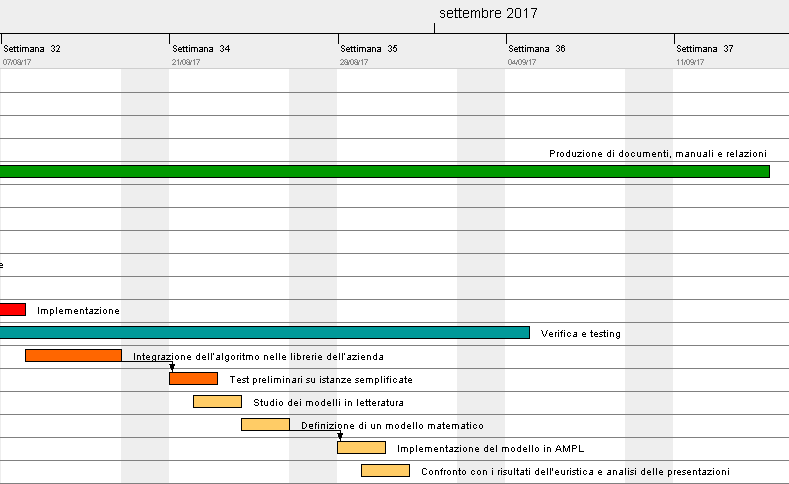
\includegraphics[width=14.9cm,keepaspectratio]{../immagini/pdp_2.png}
    \caption{Diagramma di Gantt per il piano di lavoro, settimane 5-9}
    \end{widepage}
\end{figure}

\clearpage
%**************************************************************
\section{Ambiente di lavoro}
    \subsection{Metodologia di sviluppo}
    La metodologia di sviluppo adottata in \TS\ non si riconduce ad un modello in particolare, nonostante presenti delle affinità sia con il \emph{\gls{mod-incr}}\glsfirstoccur\ che con il metodo \emph{\gls{agile}}\glsfirstoccur\ di tipo \emph{\gls{scrum}}\glsfirstoccur. Infatti, per la pianificazione del lavoro a lungo termine sono stati definite delle fasi, affini idealmente a degli incrementi, associate a \emph{\gls{milestone}}\glsfirstoccur\ ben definite; tuttavia all'interno di ogni incremento l'approccio allo sviluppo diventa più simile al metodo agile, in quanto il Project Manager, ma anche i membri del team di sviluppo stesso, ad inserire e assegnare/assegnarsi i task del backlog. Affine al metodo scrum è anche il controllo quotidiano dell'avanzamento dei lavori rappresentato dalla breve riunione mattutina con tutti i membri del team. \\
    Questa metodologia di sviluppo funziona all'interno di \TS\ poiché il team sviluppa un software per l'azienda stessa e quindi il colloquio e l'interazione fra sviluppatori e stakeholders è estremamente facilitato.

    \subsection{Gestione di progetto}
        \subsubsection{Versionamento}
        Per quanto riguarda il versionamento, l'azienda ha un \emph{\gls{repository}}\glsfirstoccur\ \emph{\gls{git}}\glsfirstoccur\ privato su Bitbucket\footnote{{\color{blue} \url{https://bitbucket.org/}}}, a cui mi è stato dato l'accesso in lettura. Il ramo master di tale repository costituisce il codice del framework e delle applicazioni aggiornato all'ultima versione e funzionante; mentre per tutte le modifiche in via di sviluppo o le estensioni, i membri del team lavorano su dei branch personali. Anche per me ne è stato creato uno, nel quale ho potuto modificare il framework e scrivere la mia applicazione.
        
        \subsubsection{Ticketing}
        Le attività da svolgere nel tempo medio-breve, che vanno a costituire il backlog, sono gestite tramite la piattaforma di project management ``Taiga''\footnote{{\color{blue} \url{https://taiga.io/}}}. I membri del team possono aggiungere attività al backlog che inizialmente ricadono nella categoria ``to do'', quando vengono assegnate a qualcuno che incomincia a occuparsene nella categoria ``In progress'' e poi successivamente in ``To test'' e ``Complete''. Alla stessa attività possono venire assegnati più membri del team.
        Anche per me è stata creata un'utenza con accesso ai ticket.
                
        \subsubsection{Altri strumenti per la gestione di progetto}
        \begin{itemize}
            \item \textbf{Google Drive}\footnote{{\color{blue} \url{https://www.google.com/intl/it\_ALL/drive/}}}: per la condivisione veloce di file come guide, documentazioni, riferimenti utili e documenti informali.
            \item \textbf{Google Calendar}\footnote{{\color{blue} \url{https://www.google.com/calendar}}}: per la gestione degli eventi ed impegni.
        \end{itemize}
    
    \subsection{Documentazione}
        Per quanto riguarda la produzione di documenti, manuali e relazioni richiesti, l'azienda non ha uno standard e mi ha dunque delegato la scelta di che software utilizzare per la loro produzione. 
        \subsubsection{Doxygen}
        Per quanto riguarda la documentazione del codice, la mia scelta è ricaduta su Doxygen\footnote{{\color{blue} \url{http://www.stack.nl/~dimitri/doxygen/}}}. Doxygen è uno strumento per la generazione di documentazione a partire dal codice commentato per molti linguaggi di programmazione, fra i quali il C\texttt{++}. Genera documentazione sia in HTML che in \LaTeX, corredandola con diagrammi delle classi ed estraendo i commenti direttamenti dai sorgenti per commentare attributi e metodi delle classi.
        \subsubsection{Diagrammi UML e Use Case}
        Per la progettazione è stato necessario modellare con UML, la mia scelta è ricaduta su Astah Professional\footnote{{\color{blue} \url{http://astah.net/editions/professional}}}, disponibile in versione gratuita grazie alla licenza accademica, perché identificato come il software più completo fra quelli dedicati. Astah Professional supporta sia i costrutti di UML 1.x che di UML 2.x e permette di modellare casi d'uso, i diagrammi delle classi, degli oggetti, delle attività e di sequenza.

    \subsection{Ambiente di sviluppo}

Il framework aziendale da estendere è programmato in C\texttt{++} ed offre una base per l'implementazione di algoritmi di ottimizzazione. Consiste di librerie per l'utilizzo di grafi, di algoritmi euristici di tipo \emph{\gls{greedy}}\glsfirstoccur\ e di meta-euristiche, ad esempio \emph{\gls{tabu}}\glsfirstoccur, che il l'estensione del framework andrà a sfruttare.

\subsubsection{IDE}
Il progetto originale è nato su Visual Studio, perciò è consigliato utilizzare tale \emph{\gls{ideg}}\glsfirstoccur\  per lo sviluppo in quanto i file di progetto con estensione \textit{.vcxproj} che contengono le informazioni necessarie alla compilazione sono già presenti.\\ Trattandosi comunque di codice scritto in C\texttt{++}, può essere utilizzato qualsiasi IDE ne fornisca il supporto.

\subsubsection{Sistemi operativi}
Poiché il progetto è nato su Visual Studio, la scelta più naturale per il sistema operativo di scelta è rappresentata da Windows; ciononostante i membri possono lavorare indifferentemente anche su Linux o Mac OS.

%**************************************************************
\newpage
\section{Analisi preventiva dei rischi}
Nella seguente tabella viene riportata l'analisi dei rischi in cui si può incorrere nel corso del progetto.\\
Nel {\hyperref[cap:conclusioni]{settimo capitolo}}
è riportata un'attualizzazione dei rischi che si sono effettivamente verificati.
\begin{table}[!htb]
    \setlength\extrarowheight{5pt}
    \caption{Analisi preventiva dei rischi}
    \label{tab:richio}
    \begin{tabularx}{\textwidth}{
            |p{\dimexpr.40\linewidth-2\tabcolsep-1.3333\arrayrulewidth}% column 1
            |p{\dimexpr.40\linewidth-2\tabcolsep-1.3333\arrayrulewidth}% column 2
            |p{\dimexpr.20\linewidth-2\tabcolsep-1.3333\arrayrulewidth}|% column 3
        }
        \hline
        \thead{Descrizione} & \thead{Trattamento} & \thead{Rischio}\\
        \hline
        
        \multirow{2}{*}{\shortstack[l]{Scelte di bad design nella\\ progettazione del framework\\ aziendale esistente, che possono\\ rendere difficoltosa l'estensione.}}  & \multirow{2}{*}{\shortstack[l]{Se verificato, si potrà\\ avere un confronto con gli\\ sviluppatori del framework\\ per cercare assieme una\\ soluzione.}} & Occorrenza: Alta \\ \cline{3-3}
        &  & Pericolosità: Medio-Alta \\
        \hline
        
        \multirow{2}{*}{\shortstack[l]{Bug all'interno del framework \\ poiché alcune sue parti si \\ trovano ancora in fase di \\sviluppo.}}  & \multirow{2}{*}{\shortstack[l]{Se verificato, si potrà\\ avere un confronto con gli\\ sviluppatori del framework\\ per cercare assieme una\\ soluzione.}} & Occorrenza: Bassa \\ \cline{3-3}
        &  & Pericolosità: Alta \\
        \hline
    \end{tabularx}
\end{table}%

